\section{Results}\label{sec:results}
\subsection{DESI imaging LRG sample}

Fig. \ref{fig:cl_dr9} shows the measured power spectrum of the DESI imaging DR9 LRG sample before and after applying imaging weights, the best fit theory curves, and the mean power spectrum and 1$\sigma$ error estimated from the $\fnl=0$ lognormal simulations. The power spectra are similar on small scales ($\ell > 20$), but the differences between various cleaning methods are significant on large scales. By comparing \textit{linear conservative I} to \textit{linear conservative II}, we find that the measure power spectra on modes with $6\leq \ell < 10$ are noticeably different between the two methods. We associate the differences to the r-band psfsize template in \textit{linear conservative II}. On other scales, the differences between the spectra after the linear-based cleaning are negligible, supporting the idea that our feature selection procedure has worked to identify the primary maps causing excess clustering signal. Comparing \textit{nonlinear conservative II} to \textit{linear conservative II}, we find that the measured spectra on $4 \leq \ell < 6$ are very different, probably pointing at nonlinear spurious fluctuations with large-scale characteristics due to the extinction. Adding stellar density to the nonlinear approach (\textit{nonlinear conservative II + nStar}) results in less excess power relative to the mock power spectrym, with the modes on $2\leq \ell < 4$ reflecting the biggest change. The flexibility of the nonlinear approach to correct for these effects ameliorates the clustering measurements on these scales.

\begin{figure}
    \centering
    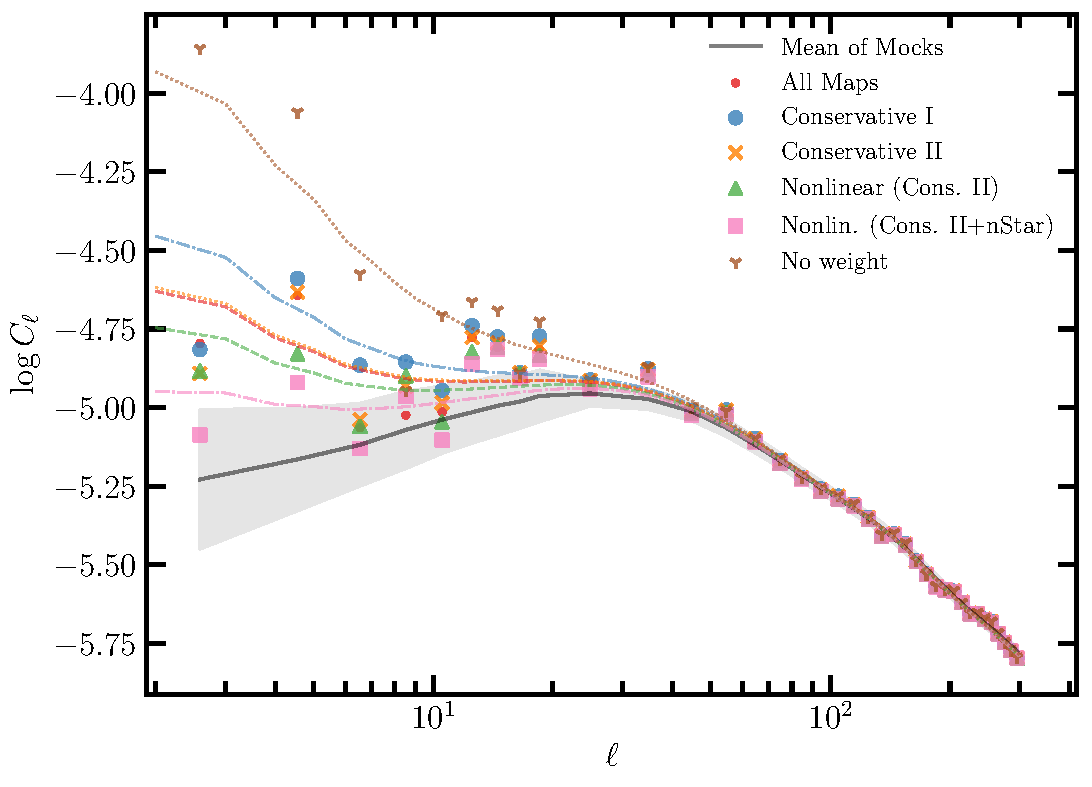
\includegraphics[width=0.48\textwidth]{figures/model_dr9.pdf} 
    \caption{The angular power spectrum of the DR9 LRG sample before (\textit{No weight}) and after correcting for imaging systematics using various methods with their corresponding best fit theory curves. The shade represents $1\sigma$ error constructed from the $\fnl=0$ mocks.}
    \label{fig:cl_dr9}
\end{figure}

\subsubsection{Calibrated constraints}

\begin{figure}
    \raggedleft
    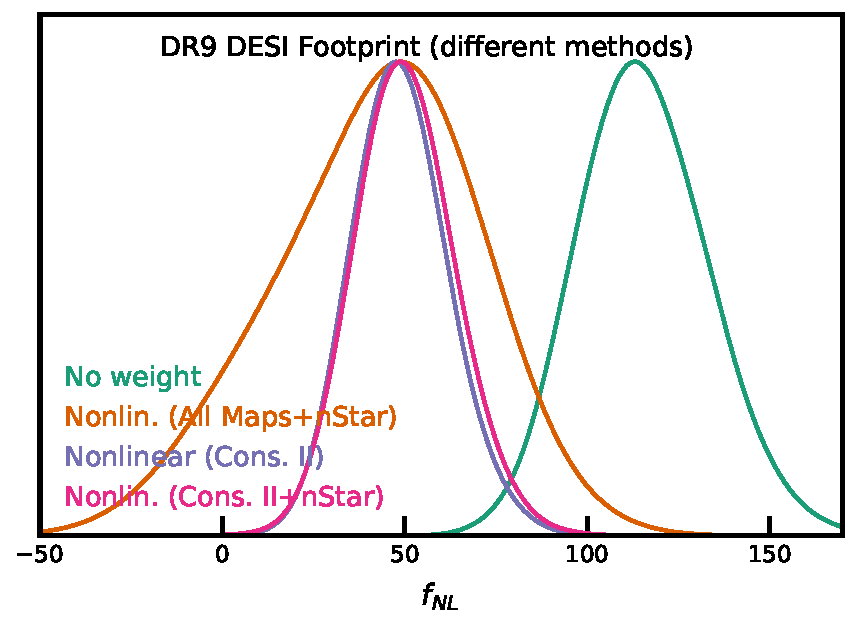
\includegraphics[width=0.424\textwidth]{mcmc_dr9methods1d.pdf}
    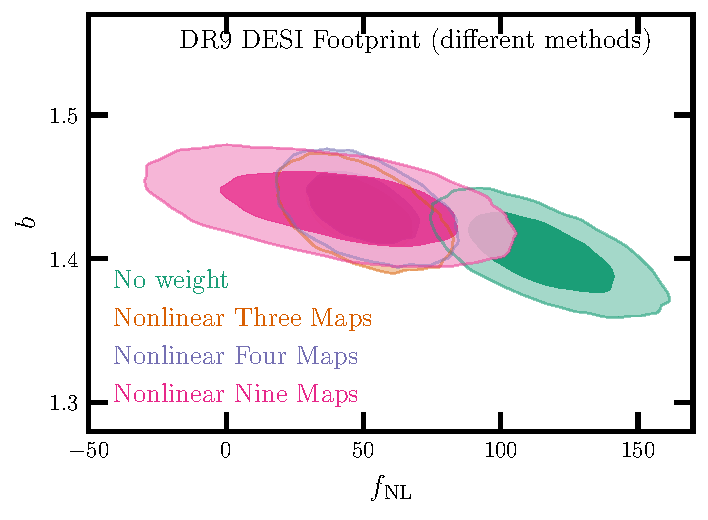
\includegraphics[width=0.45\textwidth]{figures/mcmc_dr9methods.pdf} 
    \caption{Calibrated constrains from the DR9 LRG sample. \textit{Top}: probability distribution for $\fnl$ marginalized over the shotnoise and bias. \textit{Bottom}: $68\%$ and $95\%$ probability distribution contours for the bias and $\fnl$ from the DR9 LRG sample before and after applying nonlinear cleaning methods. The lognormal mocks are used to correct these distributions for mitigation bias.}\label{fig:mcmc_dr9}
\end{figure}

\begin{table*}
    \caption{Calibrated best fit and marginalized mean estimates for $\fnl$ from fitting power spectrum of the DESI DR9 LRG sample before and after correcting for systematics. Degree of freedom is 34 (37 data points - 3 parameters).}
    \label{tab:dr9methodcalib}
   \centerline{%     
    \begin{tabular}{llllllll}
    \hline
    \hline
   &  & 	  & & $\fnl$ &  &  \\
   \cmidrule(r{.7cm}){3-6}
Footprint                               & Method & 	Best fit  & Mean & $ 68\%$ CL & $ 95\%$ CL & $\chi^{2}$ \\
    \hline
DESI                      & No Weight   & $113.18$& $115.49$& $ 98.14<\fnl<132.89$& $ 83.51<\fnl<151.59$ &   44.4\\
DESI                      & Nonlinear (Cons. II)& $ 47.38$& $ 48.81$& $ 36.08<\fnl< 61.44$& $ 25.03<\fnl< 75.64$ &   34.6\\
DESI                      & Nonlin. (Cons. II+nStar)& $ 48.92$& $ 50.10$& $ 36.88<\fnl< 63.31$& $ 24.87<\fnl< 77.78$ &   35.2\\
DESI                      & Nonlin. (All Maps+nStar)& $ 49.69$& $ 41.91$& $ 13.10<\fnl< 69.14$& $-15.96<\fnl< 91.84$ &   39.5\\
   \hline
    \end{tabular}
}
\end{table*}

All $\fnl$ constraints presented here are calibrated for the effect of mitigation bias using the lognormal simulations. Tab. \ref{tab:dr9methodcalib} describes the best fit and marginalized mean estimates of $\fnl$ from fitting the power spectrum of the DR9 LRG sample before and after cleaning with the nonlinear approach given various combinations of imaging templates. Fig \ref{fig:mcmc_dr9} shows the marginalized probability distribution for $\fnl$ (top) and the $68\%$ and $95\%$ probability contours for the bias parameter and $\fnl$ from the DR9 sample before (\textit{no weight}) and after applying various imaging weights. With the imaging weights applied, we obtain $36.08 (25.03) < \fnl < 61.44(75.64)$ with $\chi^{2}=34.6$ for \textit{nonlinear conservative II}, $36.88(24.87) < \fnl < 63.31(77.78)$ with $\chi^{2}=35.2$ for \textit{nonlinear conservative II + nStar}, and $13.10(-15.96) < \fnl < 69.14(91.84)$ with $\chi^{2}=39.5$ for \textit{nonlinear all maps + nStar} at $68\% (95\%)$ confidence over 34 degrees of freedom. Overall, we find the maximum likelihood estimates to be consistent between among the various cleaning methods. For the conservative methods, the confidence intervals with or without $nStar$ are consistent and more than $3\sigma$ off from zero. The method \textit{nonlinear all maps+nStar} has asymmetric probability distribution, a larger uncertainty, and consistent with $\fnl=0$ within the $95\%$ confidence interval. For comparison, we obtain $98.14(83.51) < \fnl < 132.89(151.59)$ at $68\% (95\%)$ confidence with $\chi^{2}=44.4$ for the \textit{no weight} approach. The uncalibrated probability contours are presented in Appendix \ref{sec:dr9uncalib}.


\subsubsection{Robustness tests}
Now we proceed to perform some robustness tests and assess how sensitive the $\fnl$ constraints are to the assumptions made in the analysis or the quality cuts applied to the data.  The calibration of mitigation bias for all of these runs is beyond the scope of this work. Therefore, the constraints presented here are subject to the mitigation bias effect. Table \ref{tab:dr9method} describes the uncalibrated $\fnl$ constraints from the DR9 LRG sample. Our tests are as follows:

\begin{table*}
    \caption{Uncalibrated best fit and marginalized mean estimates for $\fnl$ from fitting power spectrum of the DR9 LRG sample before and after correcting for systematics. Degree of freedom is 34 (37 data points - 3 parameters).}
    \label{tab:dr9method}
   \centerline{%     
    \begin{tabular}{llllllll}
    \hline
    \hline
   &  & 	  & & $\fnl$ &  &  \\
   \cmidrule(r{.7cm}){3-6}
Footprint                               & Method & 	Best fit  & Mean & $ 68\%$ CL & $ 95\%$ CL & $\chi^{2}$ \\
    \hline
DESI                                    & No Weight   & $113.18$& $115.49$& $ 98.14<\fnl<132.89$& $ 83.51<\fnl<151.59$ &   44.4\\
DESI                                    & Linear (All Maps)& $ 36.05$& $ 37.72$& $ 26.13<\fnl< 49.21$& $ 16.31<\fnl< 62.31$ &   41.1\\
DESI                                    & Linear (Conservative I)& $ 49.58$& $ 51.30$& $ 38.21<\fnl< 64.33$& $ 27.41<\fnl< 78.91$ &   38.8\\
DESI                                    & Linear (Conservative II)& $ 36.63$& $ 38.11$& $ 26.32<\fnl< 49.86$& $ 16.36<\fnl< 63.12$ &   39.6\\
DESI                                    & Nonlinear (Cons. II)& $ 28.58$& $ 29.79$& $ 18.91<\fnl< 40.59$& $  9.47<\fnl< 52.73$ &   34.6\\
DESI                                    & Nonlin. (Cons. II+nStar)& $ 16.63$& $ 17.52$& $  7.51<\fnl< 27.53$& $ -1.59<\fnl< 38.49$ &   35.2\\
DESI                                    & Nonlin. (All Maps+nStar)& $ -5.87$& $ -9.19$& $-21.45<\fnl<  2.40$& $-33.81<\fnl< 12.06$ &   39.5\\
DESI (imag. cut)                  & Nonlin. (Cons. II)& $ 29.16$& $ 30.57$& $ 19.05<\fnl< 42.18$& $  9.01<\fnl< 54.81$ &   35.8\\
DESI (comp. cut)                 & Nonlin. (Cons. II)& $ 28.07$& $ 29.48$& $ 18.38<\fnl< 40.50$& $  8.81<\fnl< 53.10$ &   34.5\\
DESI                                    & Nonlin. (Cons. II)+Cov& $ 31.62$& $ 33.11$& $ 20.94<\fnl< 45.24$& $ 10.56<\fnl< 59.16$ &   33.5\\
\hline
BASS+MzLS                        & Nonlin. (Cons. II)& $ 15.43$& $ 19.01$& $ -1.17<\fnl< 39.43$& $-19.19<\fnl< 63.56$ &   35.6\\
BASS+MzLS                        & Nonlin. (Cons. II+nStar)& $ 13.12$& $ 15.39$& $ -4.59<\fnl< 35.56$& $-24.88<\fnl< 59.31$ &   34.7\\
BASS+MzLS                        & Nonlin. (All Maps+nStar)& $ -3.73$& $ -6.34$& $-27.11<\fnl< 13.75$& $-47.44<\fnl< 33.94$ &   36.8\\
BASS+MzLS (imag. cut)      & Nonlin. (Cons. II)& $ 25.03$& $ 29.12$& $  6.16<\fnl< 52.44$& $-14.22<\fnl< 80.54$ &   36.2\\
BASS+MzLS (comp. cut)     & Nonlin. (Cons. II)& $ 16.99$& $ 20.90$& $  0.26<\fnl< 41.76$& $-18.30<\fnl< 67.12$ &   35.8\\
DECaLS North                     & Nonlin. (Cons. II)& $ 41.02$& $ 44.89$& $ 23.33<\fnl< 66.78$& $  4.96<\fnl< 93.02$ &   41.1\\
DECaLS North                     & Nonlin. (Cons. II+CALIBZ+HI)& $ 55.46$& $ 60.44$& $ 36.78<\fnl< 84.05$& $ 17.86<\fnl<112.81$ &   38.4\\
DECaLS North                     & Nonlin. (Cons. II+nStar)& $ 31.45$& $ 34.78$& $ 14.14<\fnl< 55.79$& $ -5.81<\fnl< 80.80$ &   41.2\\
DECaLS North                     & Nonlin. (All Maps+nStar)& $  0.81$& $ -5.68$& $-29.73<\fnl< 16.71$& $-53.15<\fnl< 36.19$ &   45.1\\
DECaLS North (no DEC cut)      & Nonlin. (Cons. II)& $ 41.05$& $ 44.82$& $ 23.58<\fnl< 66.08$& $  6.40<\fnl< 91.42$ &   40.7\\
DECaLS North (imag. cut)   & Nonlin. (Cons. II)& $ 43.27$& $ 48.39$& $ 24.60<\fnl< 72.50$& $  4.71<\fnl<101.42$ &   35.1\\
DECaLS North (comp. cut)  & Nonlin. (Cons. II)& $ 40.55$& $ 44.63$& $ 22.41<\fnl< 67.11$& $  3.95<\fnl< 94.06$ &   41.4\\
DECaLS South                    & Nonlin. (Cons. II)& $ 31.24$& $ 33.21$& $ 14.89<\fnl< 52.40$& $ -5.11<\fnl< 74.35$ &   30.2\\
DECaLS South                    & Nonlin. (Cons. II+CALIBZ+HI)& $ 33.79$& $ 37.50$& $ 17.71<\fnl< 57.42$& $ -0.31<\fnl< 80.94$ &   30.8\\
DECaLS South                    & Nonlin. (Cons. II+nStar)& $ 14.34$& $  6.28$& $-21.19<\fnl< 30.01$& $-53.63<\fnl< 49.51$ &   31.9\\
DECaLS South                    & Nonlin. (All Maps+nStar)& $-36.76$& $-32.01$& $-49.38<\fnl<-13.61$& $-65.26<\fnl<  7.52$ &   31.5\\
DECaLS South (no DEC cut) & Nonlin. (Cons. II)& $ 43.79$& $ 46.79$& $ 30.16<\fnl< 63.41$& $ 16.38<\fnl< 82.72$ &   23.8\\
DECaLS South (imag. cut)        & Nonlin. (Cons. II)& $ 26.47$& $ 23.36$& $  3.18<\fnl< 47.84$& $-57.69<\fnl< 71.39$ &   30.0\\
DECaLS South (comp. cut)       & Nonlin. (Cons. II)& $ 29.62$& $ 31.76$& $ 13.00<\fnl< 51.58$& $ -9.78<\fnl< 74.28$ &   29.7\\
   \hline
    \end{tabular}
}
\end{table*}

\begin{itemize}
\item \textbf{Imaging regions}: First, we compare how the $\fnl$ constraints from fitting the power spectrum of the whole DESI footprint compares to that from the power spectrum for each sub-survey individually, namely BASS+MzLS, DECaLS North, and DECaLS South. Fig. \ref{fig:mcmc_dr9reg} shows $68\%$ and $95\%$ probability contours on $\fnl$ and $b$ from each individual survey or DESI. The cleaning method here is \textit{nonlinear conservative II}. Overall, we find that the constraints from all imaging surveys are consistent with each other within $68\%$ confidence. Both BASS+MzLS and DECaLS South yield constraints consistent with $\fnl=0$ within $95\%$, but DECaLS North deviates from zero PNG at more than $2\sigma$. 

\item \textbf{Stellar density template (\textit{nStar})}: Adding the stellar density template (\textit{nonlinear conservative II+ nStar}) does not change the constraints from BASS+MzLS much, but it shifts the $\fnl$ distributions to lower values in DECaLS North and DECaLS South by $0.5\sigma$ and $\sigma$, respectively, reconciling all constraints with $\fnl=0$. This might indicate that there are either some unresolved issues with the stellar contamination in DECaLS North and DECaLS South. Although our mock test indicates that we could expect a mitigation bias around $\Delta \fnl \sim 10-16$. So we can argue that some of the shift in constraints can be associated with the fact that the stellar density template is correlating with large-scale structure. We note that differences are more significant when all maps and stellar density are used as input. This is expected as cleaning the data with more maps is more prone to the over-correction issue.

\item \textbf{Pixel completeness (\textit{comp. cut})}: We discard pixels with $f_{\rm pix} < 0.5$ to assess the effect of partially complete pixels on $\fnl$. The $f_{\rm pix}$ cut removes only $.6\%$ of the survey area. We observe no significant shift in the $\fnl$ constraints. The impact on the best fit $\fnl$ estimate from fitting the DESI power spectrum is negligible. When applied this impact of this cut on each region separately, we find that the BASS+MzLS constraint increases by $\Delta \fnl \sim 10$ while the constraints from DECaLS North and DECaLS South do not show significant changes after this cut.

\item \textbf{Imaging quality (\textit{imag. cut})}: We remove pixels with poor imaging from the DESI footprint by applying the following cuts on imaging properties; $E[B-V]<0.1$, $nStar < 3000$, $depth_{g} > 23.2$, $depth_{r} > 22.6$, $depth_{z} > 22.5$, $psfsize_{g}<2.5$, $psfsize_{r}<2.5$, and $psfsize_{z}<2$. Overall the constraints are consistent despite best fit and marginalized mean estimates shift. Quantitatively, we lose about $8.2\%$ survey area, and the best fit $\fnl$ estimate changes about $2\%$ from $28.58$ to $29.16$. See \textit{imag cut} in Table \ref{tab:dr9method}. For BASS+MzLS only, the imaging cut increases the best fit by $62\%$ from $15.43$ to $25.03$. For DECaLS North and DECaLS South, the best fit increases by $5\%$ and $15\%$ respectively.

\item \textbf{Covariance}
We now use the mocks with $\fnl=76.92$ to construct a covariance matrix, and with the new covariance we observe a $12\%$ increase in the $\fnl$ constraint uncertainties and $11\%$ increase in the best fit estimate of $\fnl$.

\item \textbf{Lowest $\ell$} 
We decrease the largest mode (or increase the lowest $\ell$) used in estimating the best fit and $68\%$ confidence intervals. Fig. \ref{fig:mcmc_dr9elmin} illustrates the results for the DESI footprint and how they compared to BASS+MzLS, DECaLS North, or DECaLS South only results. Points represent marginalized mean estimates of $\fnl$ and errorbars represent $68$\% confidence from MCMC results.Overall we find that the constraints are robust against the largest mode.

\item \textbf{External maps} We also derive imaging weights using additional external maps for the neutral hydrogen column density (HI) and magnitude calibration errors in the z band (CALIBZ). With the new weights, we find the best fit estimates increase from $41.02$ to $55.46$ for DECaLS North and from $31.24$ to $33.79$ for DECaLS South.

\item \textbf{Declination cut} Our default analysis do not use the spurious islands in DECaLS North and DECaLS South below DEC = -30 to avoid potential calibration issues. \mr{PANASTARS are used for calibration below DEC of -30.} Without these cuts, best fit $\fnl$ estimates increase from $31.24$ to $43.79$ for DECaLS South and decrease from $41.02$ to $41.05$. This indicates that indeed there is an issue with DECaLS South below DEC of $-30$.

\end{itemize}

\begin{figure}
    \centering
    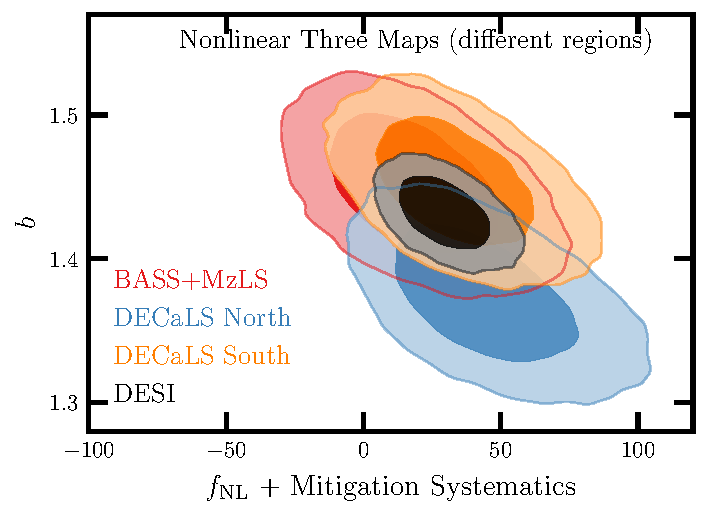
\includegraphics[width=0.45\textwidth]{figures/mcmc_dr9regions.pdf} 
    \caption{Uncalibrated 2D constraints from the DR9 LRG sample for each imaging survey compared with that for the whole DESI footprint. The dark and light shades represent the $68\%$ and $95\%$ confidence intervals, respectively.}\label{fig:mcmc_dr9reg}
\end{figure}

\begin{figure}
    \centering
    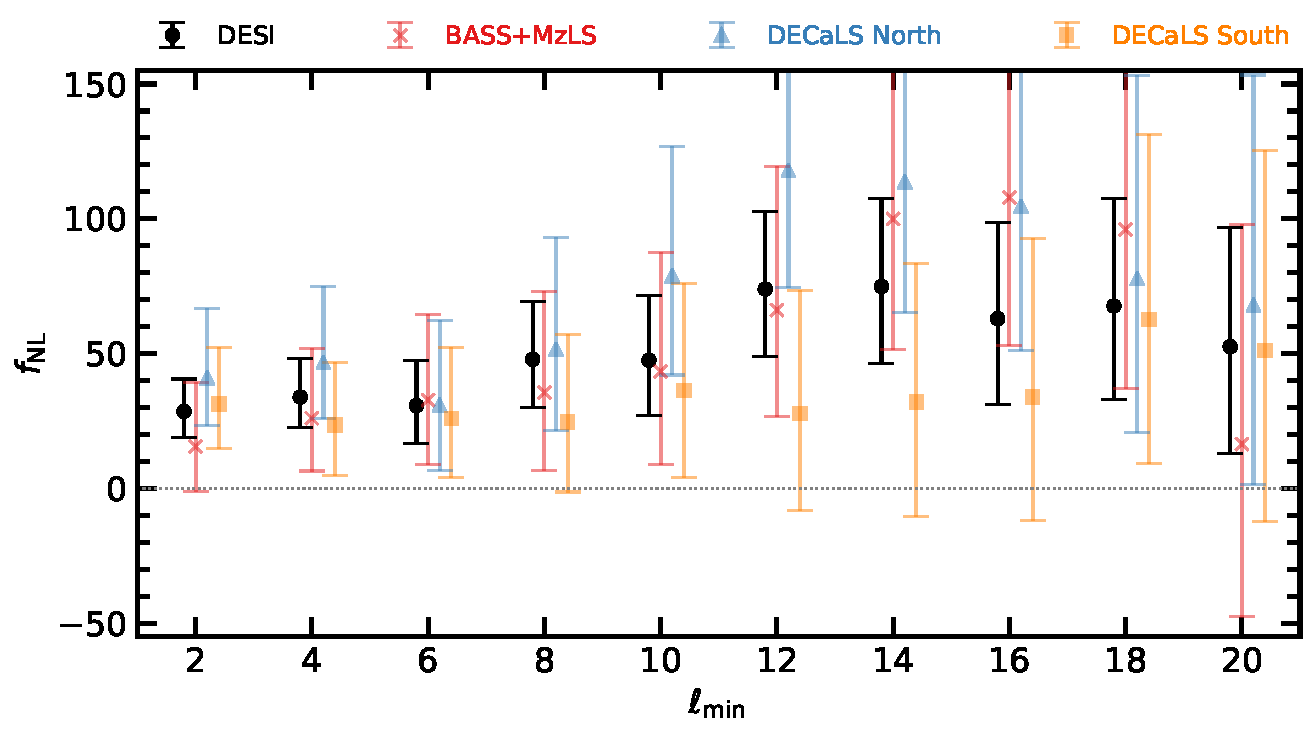
\includegraphics[width=0.45\textwidth]{figures/fnl_elmin.pdf}     
    \caption{Robustness of the uncalibrated DR9 constraints w.r.t. the largest scale (lowest $\ell$ mode) used in MCMC regression. Points represent marginalized mean estimates of $\fnl$ and errorbars represent $68$\% confidence.}\label{fig:mcmc_dr9elmin}
\end{figure}


Overall we find that the declination cut is necessary for DECaLS South, while adding external templates for HI and CALIBZ, using a different covariance, or applying imaging and completeness cuts do not alter the constraints significantly.